\section{Технический проект}
\subsection{Общая характеристика организации решения задачи}

Необходимо спроектировать и разработать приложение, которое обеспечит функционирование СКУД на круизном лайнере AIDABlu.

Приложение представляет собой панель управления, представляющую набор взаимосвязанных таблиц в базе данных системы. Панель содержит текстовую и графическую информацию (TreeView).

Приложение является десктопным, т.е. располагается и запускается внутри лишь одной операционной системы. Каждое окно приложения (за исключением главного) – это панель управления для конкретной таблицы базы данных. Приложение написано на языке Python v3.10. Управление таблицами БД реализовано с помощью библиотеки sqlite3 и SQL -- языка структурированных запросов к базе данных.

\subsection{Общие сведения о программно-информационной системе}

Полное наименование системы: Программное обеспечение для системы контроля и управления доступом на круизном судне.

Краткое обозначение системы: \textquotedbl СКУД на круизном лайнере \textquotedbl.

Описание системы: \textquotedbl СКУД на круизном лайнере \textquotedbl предназначена для корпораций, организующих круизные путешествия, предоставляя им платформу для удобного контроля и управления данными всей бизнес-системы круизного лайнера на время поездки. Система создана для обеспечения комфортной и безопасной поездки каждого пассажира и функционирования даже в форс-мажорных ситуациях.

Условия эксплуатации: \textquotedbl СКУД на круизном лайнере \textquotedbl предназначена для использования как в нормальных, так и в чрезвычайных условиях работы.

Архитектура системы: Программное обеспечение основано на десктопной архитектуре, используя современные технологии разработки, включая TKinter для Front-End части и sqlite3 для реализации запросов к БД в Back-End. Система использует базу данных SQLite.

Технологии и инструменты: В разработке использовались tkinter, sqlite3, asyncio, time

\subsection{Обоснование выбора технологии проектирования}

\subsubsection{Описание используемых технологий и языков программирования}

В процессе разработки приложения используются программные средства и языки программирования. Каждое программное средство и каждый язык программирования применяется для круга задач, при решении которых они необходимы.

\subsubsection {tkinter}
Выбор tkinter для Front-End обосновывается его простотой и кроссплатформенной поддержкой, а также минимальными требованиями к интерфейсу в пользу быстродействия. 

Пакет tkinter («интерфейс Tk») - это интерфейс Python для создания GUI. Tkinter доступен на большинстве платформ Unix, включая macOS, а также на системах Windows.

Tkinter входит в состав большинства инсталляций Python, что делает его легкодоступным для разработчиков, которые хотят создавать приложения с графическим интерфейсом, не требуя дополнительных инсталляций или библиотек.

\subsubsection {SQLite}
Выбор SQLite в качестве системы управления базами данных также обосновывается его удобством как на этапе проектирования, так и на этапе реализации.

SQLite - это библиотека на языке C, которая предоставляет легкую дисковую базу данных, не требующую отдельного серверного процесса и позволяющую обращаться к базе данных с помощью нестандартного варианта языка запросов SQL. Некоторые приложения могут использовать SQLite для внутреннего хранения данных. Также можно создать прототип приложения с использованием SQLite, а затем перенести код на более крупную базу данных, такую как PostgreSQL или Oracle.

\subsubsection {asyncio и time}
Модули asyncio и time были использованы для актуализации работы системы в реальном времени и многопоточном режиме.


\subsubsection{Язык структурированных запросов к базе данных SQL}
SQL - это стандартизированный язык программирования, который используется для управления реляционными базами данных и выполнения различных операций над данными в них. 

SQL используется для следующего:
\begin{itemize}
	\item изменение структуры таблиц и индексов базы данных;
	\item добавление, обновление и удаление строк данных;
	\item извлечение подмножеств информации из реляционных систем управления базами данных (РСУБД).
\end{itemize}


\subsubsection{Язык программирования Python}

\paragraph{Достоинства языка Python}
Python - очень продуктивный язык. Благодаря простоте Python разработчики могут сосредоточиться на решении проблемы. Написание кода экономит время и освобождает его для более ёмкой работы с другими составляющими проекта.

Python поставляется под лицензией OSI с открытым исходным кодом. Это делает его свободным для использования и распространения. Можно загружать исходный код, изменять его и даже распространять свою версию Python. Это полезно для организаций, которые хотят изменить некоторые специфические функции и использовать свою версию для разработки.

Стандартная библиотека Python огромна, в ней можно найти практически все функции, необходимые для решения любой задачи. Таким образом, не придется зависеть от внешних библиотек.

Во многих языках, таких как C/C++, для запуска программы на разных платформах необходимо изменять код. С Python дело обстоит иначе. Вы пишете один раз и запускаете программу в любом месте.

\paragraph{Недостатки языка Python}

Язык программирования Python использует большой объем памяти. Это может быть недостатком при создании приложений, когда мы предпочитаем оптимизацию памяти.

Python обычно используется для программирования на стороне сервера. Мы не видим Python на стороне клиента или в мобильных приложениях.

Python - динамически типизированный язык, поэтому тип данных переменной может измениться в любой момент. Переменная, содержащая целое число, в будущем может стать строкой, что может привести к ошибкам времени выполнения.

\subsection{Проектирование пользовательского интерфейса}
На основании требований к пользовательскому интерфейсу, представленных в пункте 2.3 технического задания, был разработан графический интерфейс десктопного приложения с применением python tkinter, ttk и SQLite. Этот процесс подчеркивает важность интуитивно понятного и эффективного взаимодействия с пользователем. Разработанный интерфейс ориентирован на обеспечение легкости в использовании и интуитивного понимания функционала приложения, предоставляя пользователю простое и эффективное взаимодействие с приложением.

1. Навигация по таблицам: Реализация функции навигации на основе полей psr\underline{ }btn, psr\underline{ }ua\underline{ }btn, drs\underline{ }btn, rms\underline{ }btn, pns\underline{ }btn;

2. Отдельные интерфейсы для каждой таблицы с полями: диверсификация интерфейсов происходит на основе метода show\underline{ }table;

3. Отображение текущей таблицы в реальном времени: актуальность этого графического элемента (дерева) поддерживается за счёт методов TreeRefresh и TreeCreate;

4. Возможность так или иначе воздействовать на внесённые данные базы внутри приложения: Добавление, изменение или удаление элементов реализованы в методах add\underline{ }element, update\underline{ }element и delete\underline{ }element соответственно, внутри которых формирование строк запросов к БД реализовано с помощью класса Utils.

5. Понятная навигация и лёгкий поиск среди элементов конкретной таблицы: Пользователь может переходить по элементам последовательно (метод MoveTo класса main), или же использовать отдельное текстовое поле для метода search\underline{ }element, перейдя сразу к искомому элементу таблицы.

6. Отображение локального времени: Учитывая специфику проекта -- систему для круизного лайнера, учтём, что часовой пояс может измениться во время путешествия. На уровне python и SQL была установлена привязка к локальному времени (localtime), а функционал часов запущен в асинхронном потоке во избежание ошибок и помех работы основной системы.

\subsection{Диаграмма компонентов и схема обмена данными между файлами компонента}

Диаграмма компонентов описывает особенности физического представления разрабатываемой системы. Она позволяет определить архитектуру системы, установив зависимости между программными компонентами, в роли которых может выступать как исходный, так и исполняемый код. Основными графическими элементами диаграммы компонентов являются компоненты, интерфейсы, а также зависимости между ними. На рисунке \ref{comp:image} изображена диаграмма компонентов для проектируемой системы. Она включает в себя сервер с операционной системой, на которой установлена система управления содержимым, включающая в себя базу данных и интерфейс. Помимо этого на диаграмме изображен клиентский компьютер с операционной системой, на которой установлен браузер.

\begin{figure}[ht]
\center{\includegraphics[width=1\linewidth]{comp}}
\caption{Диаграмма компонентов}
\label{comp:image}
\end{figure}

Любой компонент должен быть вызван в сценарии страницы web-сайта. Web-страница передает данные компоненту в момент вызова последнего.

На рисунке \ref{data:image} представлена схема обмена данными между сценариями компонента при вызове компонента на странице сайта.

\begin{figure}[ht]
\center{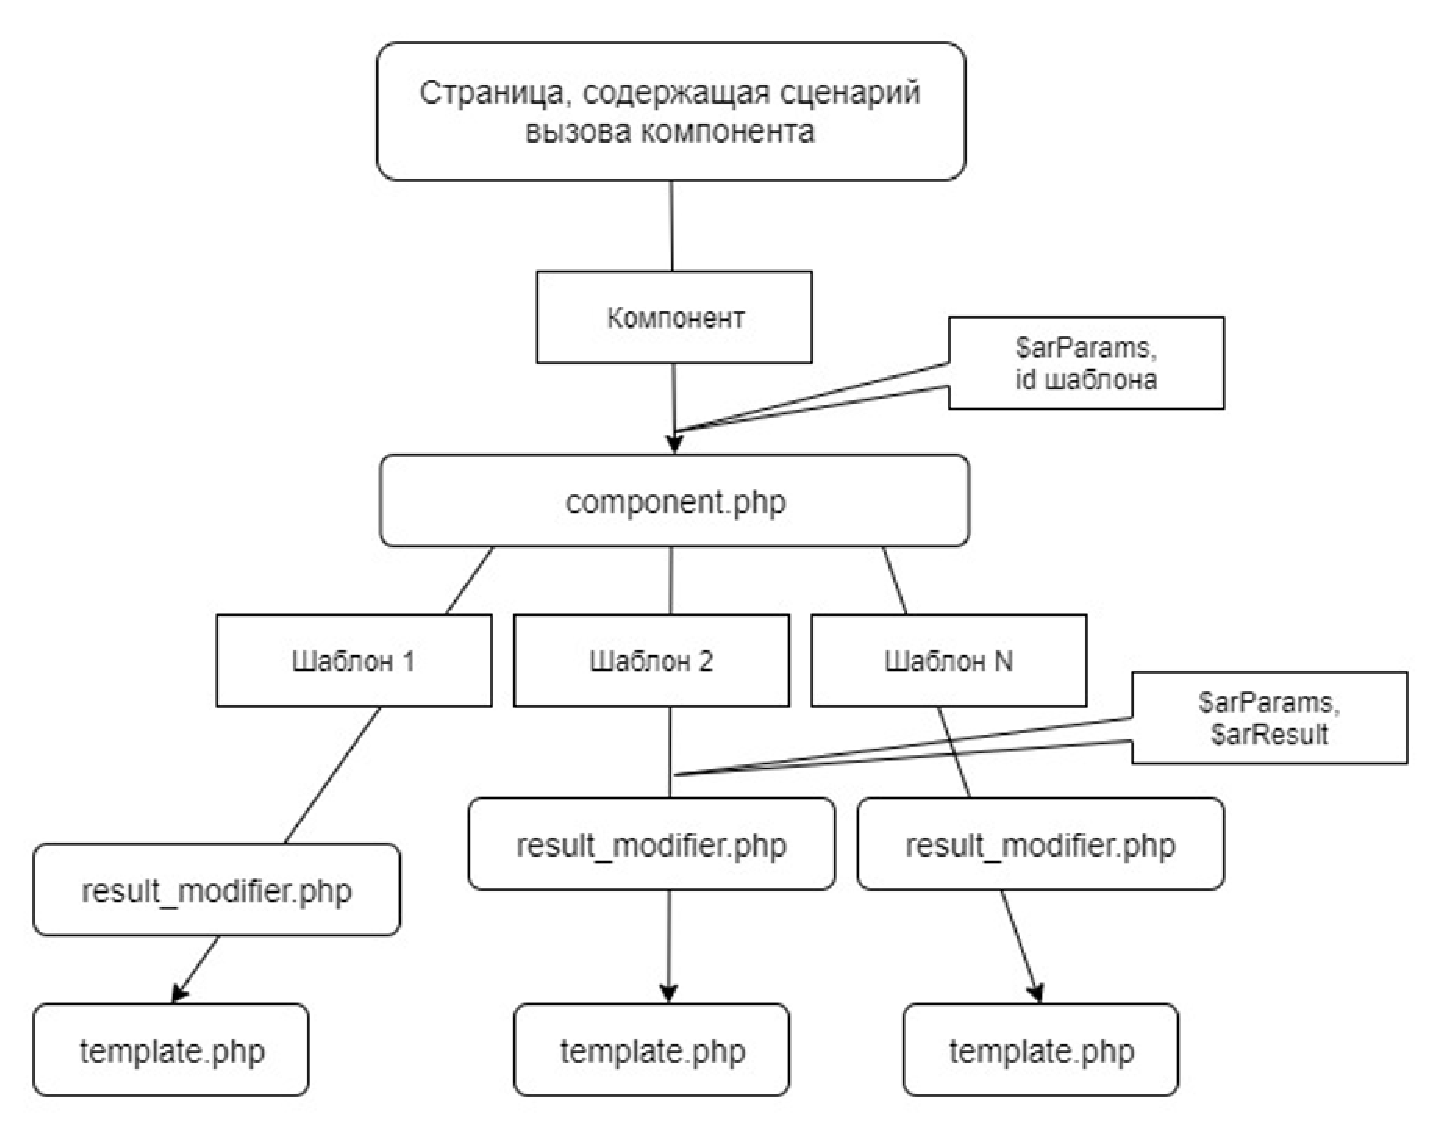
\includegraphics[width=1\linewidth]{data}}
\caption{Диаграмма компонентов}
\label{data:image}
\end{figure}

При вызове компонента в сценарии web-страницы указываются значения параметров компонента, которые далее посредством массива \$arParams передаются в сценарий файла component.php.

В сценарии файла component.php посредством метода \linebreak IncludeComponentTemplate класса CBitrixComponent происходит вызов одного из шаблонов компонента. Id шаблона также определяется в сценарии страницы web-приложения и неявно для разработчика передается указанный выше метод. Подключается сценарий файла template.php одного из шаблонов, в который передается, возможно, измененный в сценарии component.php массив \$arParams и, также, сформированный в сценарии component.php массив \$arResult. Оба этих массива доступны также и в файле result\_modifier.php, который подключается перед подключением файла template.php. 

Работа компонента заканчивается в момент завершения работы сценария файла component.php, т.е. возможно выполнить действия уже после подключения шаблона. Однако, если массив \$arResult будет изменен в сценарии шаблона, в сценарий файла компонента component.php измененные данные переданы не будут.

\subsection{Диаграмма размещения}

Диаграмма размещения (рис.~\ref{place:image}) отражает физические взаимосвязи между программными и аппаратными компонентами системы.

\vspace{-8mm} % чтобы убрать пустую строку, которая осталась после переноса рисунка на следующую страницу
\begin{figure}[ht]
\center{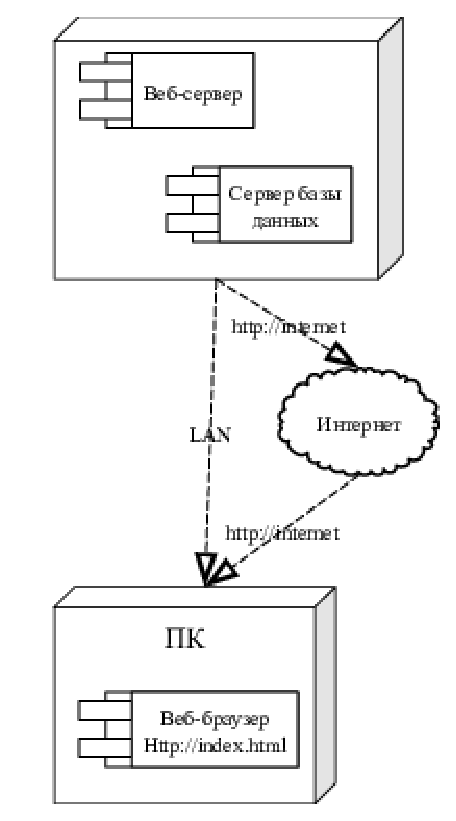
\includegraphics[width=0.57\linewidth]{place}}
\caption{Диаграмма размещения. Не помещается на страницу. Очень длинный заголовок}
\label{place:image}
\end{figure}

Она является хорошим средством для показа маршрутов перемещения объектов и компонентов в распределенной системе.

В таблице \ref{ssevsws:table} приведен пример использования пакета xltabular с автоматическим расчетом ширины столбца.

\begin{xltabular}{\textwidth}{|c|X|X|}
	\caption{Сравнение протоколов SSE и WebSocket\label{ssevsws:table}}\\ \hline
	~  & \centrow  SSE & \centrow WebSocket \\ \hline
	\endfirsthead
	\continuecaption{Продолжение таблицы \ref{ssevsws:table}}
	~ & \centrow SSE & \centrow WebSocket \\ \hline 
	\finishhead
	Направленность & 
	Однонаправленный, полудуплексный: данные посылает только сервер & 
	Двунаправленный, полнодуплексный: и сервер, и клиент могут обмениваться сообщениями \\ \hline 
	Соединение  & HTTP & WS \\ \hline 
	Тип данных & Только текст & Бинарные и текстовые данные \\ \hline 
	Доп. возможности & Встроенный механизм идентификаторов событий и переподключения & Переподключение и идентификация события реализуются на стороне приложения
\end{xltabular}

\subsection{Содержание информационных блоков. Основные сущности}

Проанализировав требования, можно выделить шесть основных сущностей:
\begin{itemize}
\item "<Новости">;
\item "<Продукция">;
\item "<Услуги">.
\end{itemize}

В состав сущности "<Новости"> можно включить атрибуты, представленные в таблице \ref{news:table}.

\begin{xltabular}{\textwidth}{|l|l|p{1.7cm}|X|}
	\caption{Атрибуты сущности "<Новости">\label{news:table}}\\ \hline
	\centrow Поле & \centrow Тип & \centrow Обяза\-тельное & \centrow Описание \\ \hline
	\thead{1} & \thead{2} & \centrow 3 & \centrow 4 \\ \hline
	\endfirsthead
	\continuecaption{Продолжение таблицы \ref{news:table}}
	\thead{1} & \thead{2} & \centrow 3 & \centrow 4 \\ \hline
	\finishhead
	\_id & ObjectId & true & Уникальный идентификатор \\ \hline 
	head & String & true & Заголовок новости \\ \hline 
	short & String & false & Аннотация к новости \\ \hline 
	createdAt & Date & true & Время создания новости \\ \hline 
	author & String & false & Автор новости \\ \hline 
	content & String & true & Текст новости \\ \hline 
	views & Integer & true & Количество просмотров новости зарегистрированными пользователями
\end{xltabular}

Пример использования различных типов столбцов представлен в таблице \ref{prod:table}. Рекомендуется использовать пакет xltabular для создания таблиц.

\begin{xltabular}{\textwidth}{|R|C{2.5cm}|l|T|}
	\caption{Атрибуты  сущности "<Новости разметки в LaTeX"> с использованием различных типов столбцов и многострочным заголовком\label{prod:table}}\\ \hline
	\centrow Поле & \centrow Тип & \centrow Обязательное & \centrow Описание \\ \hline
	\centrow 1 & \centrow 2 & \thead{3} & \centrow 4 \\ \hline
	\endfirsthead
	\continuecaption{Продолжение таблицы \ref{prod:table}}
	\centrow 1 & \centrow 2 & \thead{3} & \centrow 4 \\ \hline
	\finishhead
	\_id & ObjectId & true & Уникальный идентификатор \\ \hline 
	head & String & true & Заголовок новости \\ \hline 
	short & String & false & Аннотация к новости \\ \hline 
	createdAt & Date & true & Время создания новости \\ \hline 
	author & String & false & Автор новости \\ \hline 
	content & String & true & Текст новости \\ \hline 
	views & Integer & true & Количество просмотров новости зарегистрированными пользователями
\end{xltabular}

В системе предусмотрен внутренний механизм связи между разделами и элементами информационных блоков, поэтому введения дополнительных идентификаторов при реализации связей между сущностями не предполагается.

Экземпляры сущностей реализуются в информационных блоках посредством элементов, атрибуты сущности – посредством полей и свойств элемента. 
